\documentclass[dvipdfmx]{jarticle}
\usepackage{graphicx}
\usepackage[top=30truemm,bottom=30truemm,left=25truemm,right=25truemm]{geometry}
\usepackage{listings,jvlisting}
\usepackage{url}

\lstset{
  basicstyle={\ttfamily},
  identifierstyle={\small},
  commentstyle={\smallitshape},
  keywordstyle={\small\bfseries},
  ndkeywordstyle={\small},
  stringstyle={\small\ttfamily},
  frame={tb},
  breaklines=true,
  columns=[l]{fullflexible},
  numbers=left,
  xrightmargin=0zw,
  xleftmargin=3zw,
  numberstyle={\scriptsize},
  stepnumber=1,
  numbersep=1zw,
  lineskip=-0.5ex
}

\makeatletter
\newcommand{\subsubsubsection}{\@startsection{paragraph}{4}{\z@}%
  {1.0\Cvs \@plus.5\Cdp \@minus.2\Cdp}%
  {.1\Cvs \@plus.3\Cdp}%
  {\reset@font\sffamily\normalsize}
}
\makeatother
\setcounter{secnumdepth}{4}

\begin{document}
\begin{titlepage}
    \begin{center}
        {\huge 情報科学実験C 中間レポ―ト}
        \vspace{180pt}\\
        \begin{tabular}{rl}
            氏名 & 山久保孝亮\\
            所属 & 大阪大学基礎工学部情報科学科ソフトウェア科学コース\\
            メールアドレス & u327468b@ecs.osaka-u.ac.jp\\
            学籍番号 & 09B22084\\
            提出日 & \today\\
        \end{tabular}
    \end{center}
\end{titlepage}
\section{Tiny-ProcessorとC-Processorのデータパスの違い}
以下の図1,2はそれぞれTiny-ProcessorとC-Processorのデータパスである.
\begin{figure}[h]
  \centering
  \begin{minipage}[b]{0.49\columnwidth}
      \centering
      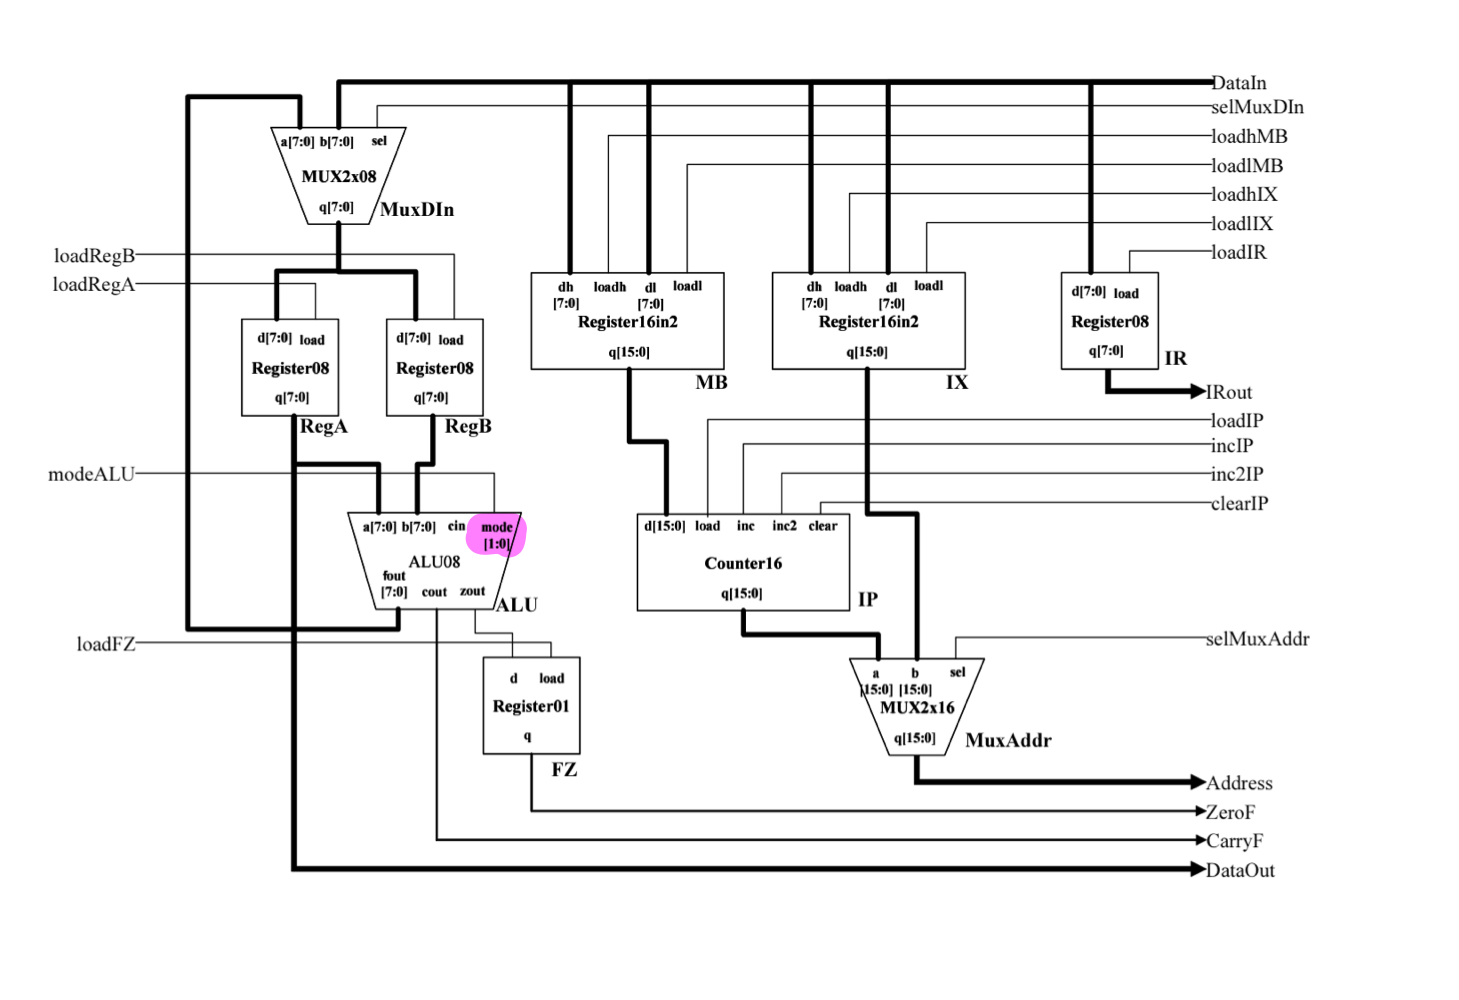
\includegraphics[width=1.1\columnwidth]{Tiny_datapath.png}
      \caption{Tiny-Processorのデータパス}
      \label{fig:a}
  \end{minipage}
  \begin{minipage}[b]{0.49\columnwidth}
      \centering
      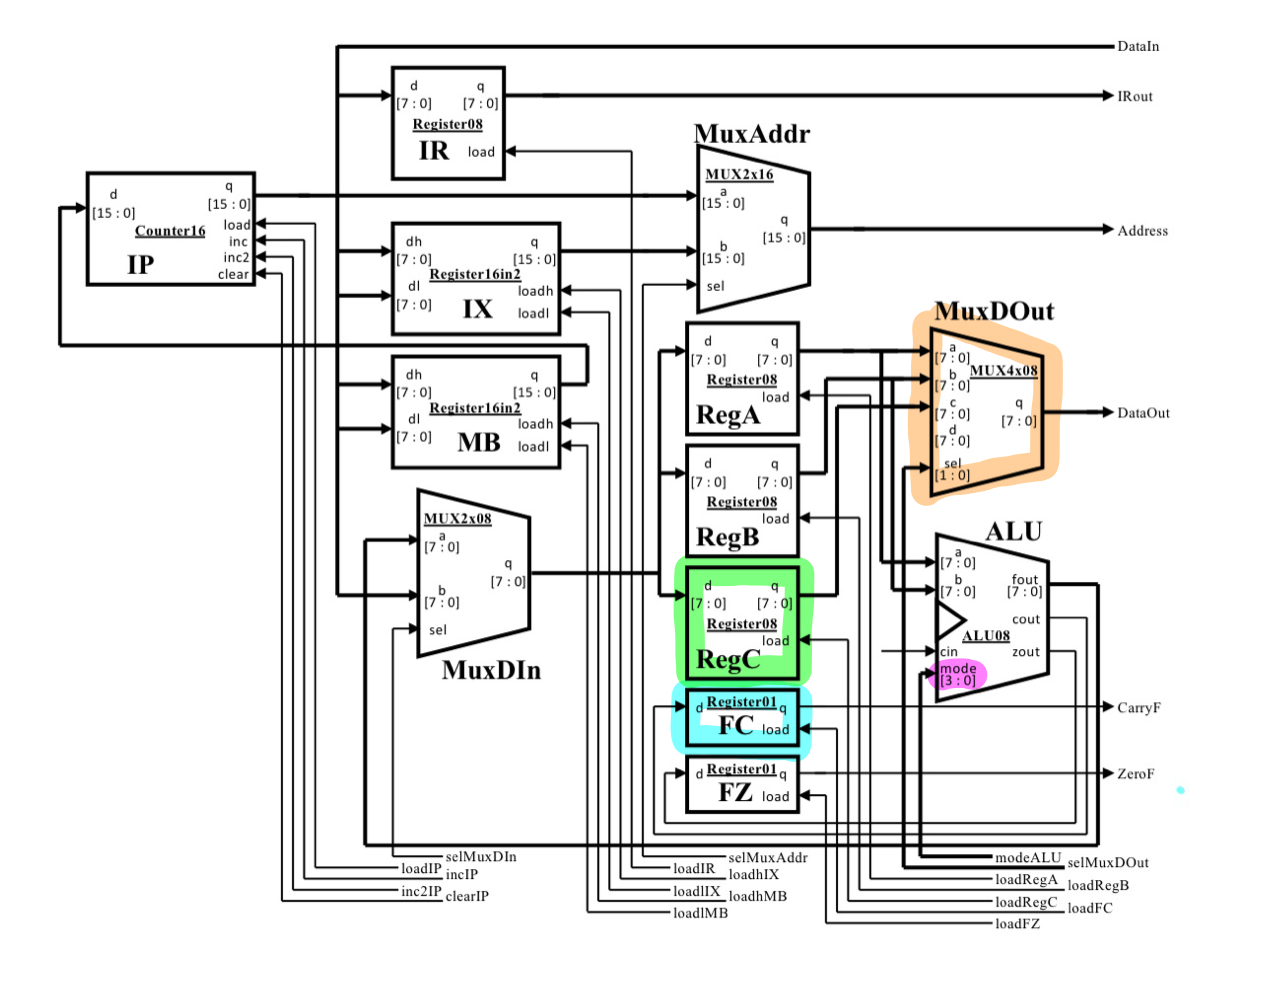
\includegraphics[width=1.1\columnwidth]{C_datapath.png}
      \caption{C-Processorのデータパス}
      \label{fig:b}
  \end{minipage}
  \end{figure}
\\この二つのデータパスの違いを明確にするために色付けをした.以下でそれぞれの違いについて述べる.
\begin{itemize}
  \item 図1のピンクに塗った部分はALUの入力modeを表す.Tiny-Processorではmodeは2ビットの入力として設計されている.図2のピンクで塗った部分は
  C-Processorの同じくALUの入力modeである.C-ProcessorではTiny-Processorよりも機能が増えており,modeの入力が4ビットに増加している.
  \item 図2の緑で塗った部分はRegCであり,C-Processorで追加されている.入力は新たに追加されたloadRegC以外はRegA,RegBと同じである.このレジスタCはSTDI命令の際に使用される.詳細な説明は2で記述する.
  \item 図2の青色で塗った部分はFCであり,C-Processorで追加されている.入力は新たに追加されたloadFCとALUの出力であるcoutで,出力はq即ちCarryFである.これはALUの演算の結果,桁上りが発生したかを判定する.これからCarryFという信号が得られ,JPC命令に利用される.
  \item 図2のオレンジで塗った部分はMuxDOutであり,4入力のマルチプレクサである.ただし,4入力の内3つしか使っておらずその3つの入力はRegA,RegB,RegCの出力である.また,4つの入力の内どの値を出力するかを決定する2ビットのselMuxDOutを追加した.
  そして出力がDataOutとなる.Tiny-ProcessorではRegAの出力がDataOutとなっていたが,C-Processorでは三つのレジスタからマルチプレクサで選択してDataOutを決定している.
\end{itemize}
\clearpage
\section{STDI命令のデータの流れ}
以下の図3は1の図2で示したC-Processorのデータパスに,STDI命令を実行する際のデータの流れを追加したものである.
\begin{figure}[h]
  \centering
  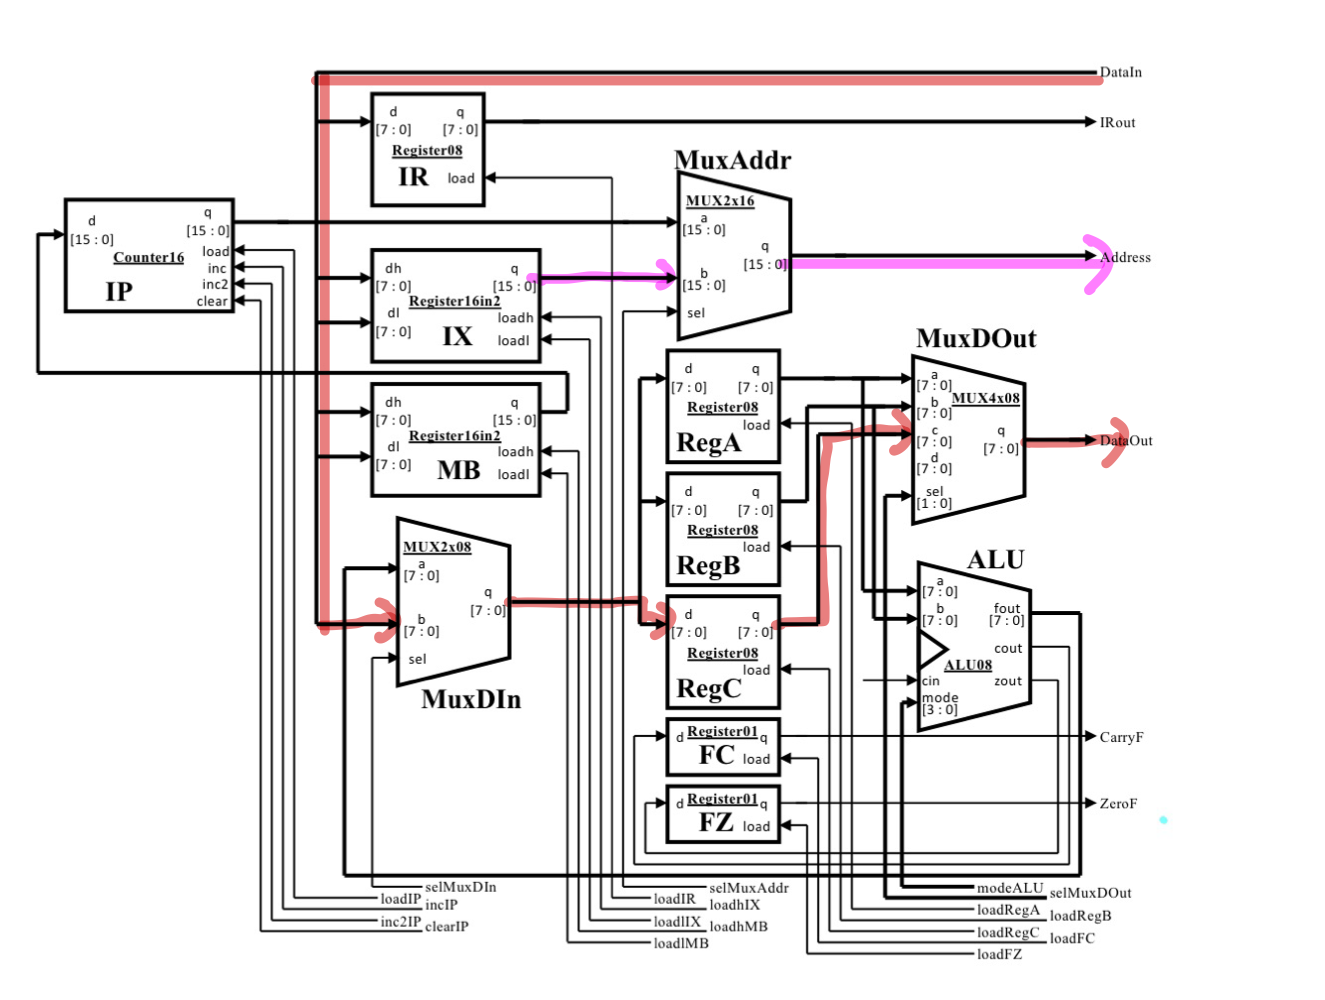
\includegraphics[width = 12cm]{STDI.png}
  \caption{C-ProcessorにおけるSTDI命令のデータの流れ}  
\end{figure}
\\ピンクの矢印はアドレス,赤の矢印はデータの流れを表している.
\section{外部出力信号用ジョンソンカウンタと内部制御信号用ジョンソンカウンタ}
設計に用いた外部出力信号のジョンソンカウンタと内部制御信号のジョンソンカウンタを示し,それぞれ説明する.
\clearpage
\subsection{外部出力用ジョンソンカウンタ}
C-Processorの外部出力用ジョンソンカウンタは以下のようになる.
\begin{figure}[h]
  \centering
  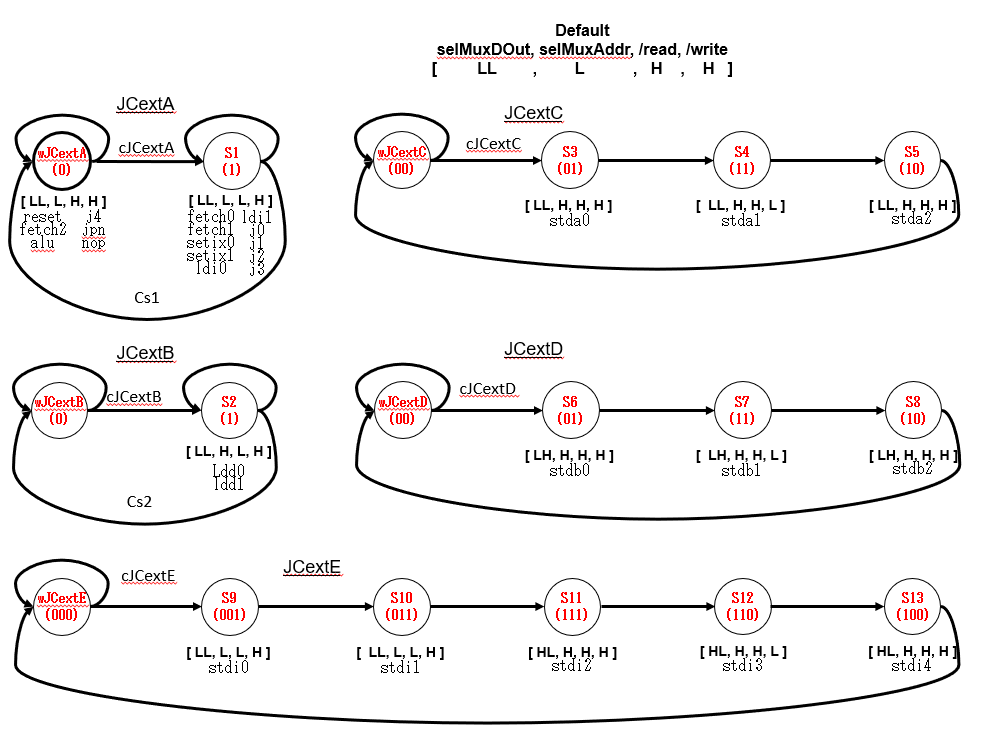
\includegraphics[width = 8cm]{ext.png}
  \caption{外部出力用ジョンソンカウンタ}
\end{figure}
\subsection{内部出力用ジョンソンカウンタ}
C-Processorの内部出力用ジョンソンカウンタは以下のようになる.
\begin{figure}[h]
  \centering
  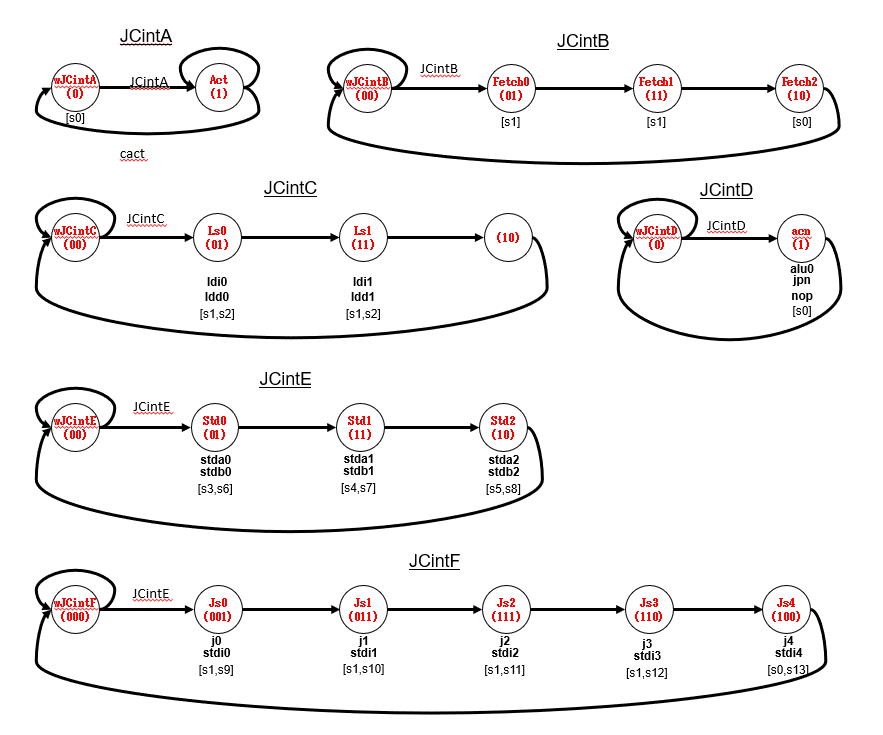
\includegraphics[width = 8cm]{int.png}
  \caption{内部出力用ジョンソンカウンタ}
\end{figure}
~\\
\section{工夫点}
C-Processorの設計にあたって,何かしらの工夫を行なったことがあれば,記述する.
拡張課題は以下の様に,それぞれの節を用意して説明する.
\section{拡張課題}
\subsection{拡張課題a:プロセッサ命令セットの拡張}
今回私が追加した命令セットは論理シフトである.いかにその仕様を示す.
\begin{table}[h]
  \centering
  \begin{tabular}{|c||c|c|c|c|}
    \hline
    命令 & オペランド & サイズ & コード\\\hline
    SLLA & id & & \\\hline
    SRLA & id & & \\\hline
    SLLB & id & & \\\hline
    SRLB & id & & \\\hline
  \end{tabular}
  \caption{追加した命令}
\end{table}
\\この4命令は,第一オペランドで即値により指定した数値分レジスタAまたはレジスタBを論理シフトするものである.
これはALUの演算の処理を切り替える4ビットのベクトルmodeALUで未使用の部分を使用して実装した.
したがって,このシフト命令を追加した後のmodeALUの処理は以下のようになる.
\begin{table}[h]
  \centering
  \begin{tabular}{|c|c|c|c|c|c|c|c|}
    \hline
    LLLL & A + B & LHLL & not A & HLLL & not B & HHLL & \\\hline
    LLLH & A - B & LHLH & A + 1 & HLLH  & B + 1 & HHLH & \\\hline
    LLHL & A and B & LHHL & A - 1 & HLHL  & B - 1 & HHHL & \\\hline
    LLHH & A or B & LHHH & id & HLHH & id & HHHH & \\\hline
  \end{tabular}
  \caption{シフト命令を追加した後のmodeALUの処理}
\end{table}
\subsection{拡張課題b:簡易アセンブラの作成}
\subsection{拡張課題c:演算機の改善}
\end{document}